\section{Introduction}
Materialized views (MVs) are a well-known approach to improving query processing performance \cite{LarsonY85, gupta1995maintenance, chirkova2011materialized, halevy2001answering}.
During the last 30 years, the research community has thoroughly studied MVs, and all major database vendors have added support for them.
In a world of ever-increasing data sizes, MVs are becoming even more important, both for traditional query processing
 \cite{lefevre2014opportunistic, bailis2014scalable, perez2014history} and for more advanced analytics based on linear algebra and machine learning \cite{nikolic2014linview, zhang2014mat}.

MVs, are effectively stored, pre-computed query results, so when the underlying data is changed, MVs can become \emph{stale}. 
Incremental view maintenance has been developed to address this problem\cite{gupta1995maintenance, chirkova2011materialized}.
Instead of re-creating an entire view for every update, incremental view maintenance executes only the incremental changes required to ensure that an MV accurately reflects the current state of the base data.   However, for frequently changing tables even incremental maintenance can be expensive; every update to the underlying data requires updating all the dependent views.  This problem is exacerbated in Big Data environments, where new records arrive at an increasingly fast rate and where data are often 
distributed across multiple machines.  As a result, in production environments it is
common to defer view maintenance to a later time \cite{chirkova2011materialized, DBLP:conf/sigmod/ColbyGLMT96}.
Deferral has many advantages such as batching updates together to amortize overheads and allowing maintenance work to be scheduled for times of low system utilization.   

While deferring maintenance has compelling benefits, it unfortunately, brings its own costs, namely that views become increasingly stale in-between maintenance periods, so that queries on those views can return increasingly incorrect results.  In a sense, stale MVs are dirty data, and queries over them suffer from inaccuracies as a result.   The observation that stale MVs are a type of dirty data leads us to the key insight behind this work, namely, that data cleaning techniques can be used to mitigate the negative impacts of deferred MV maintenance.  

\begin{figure}[t] \vspace{-1.5em}
\centering
 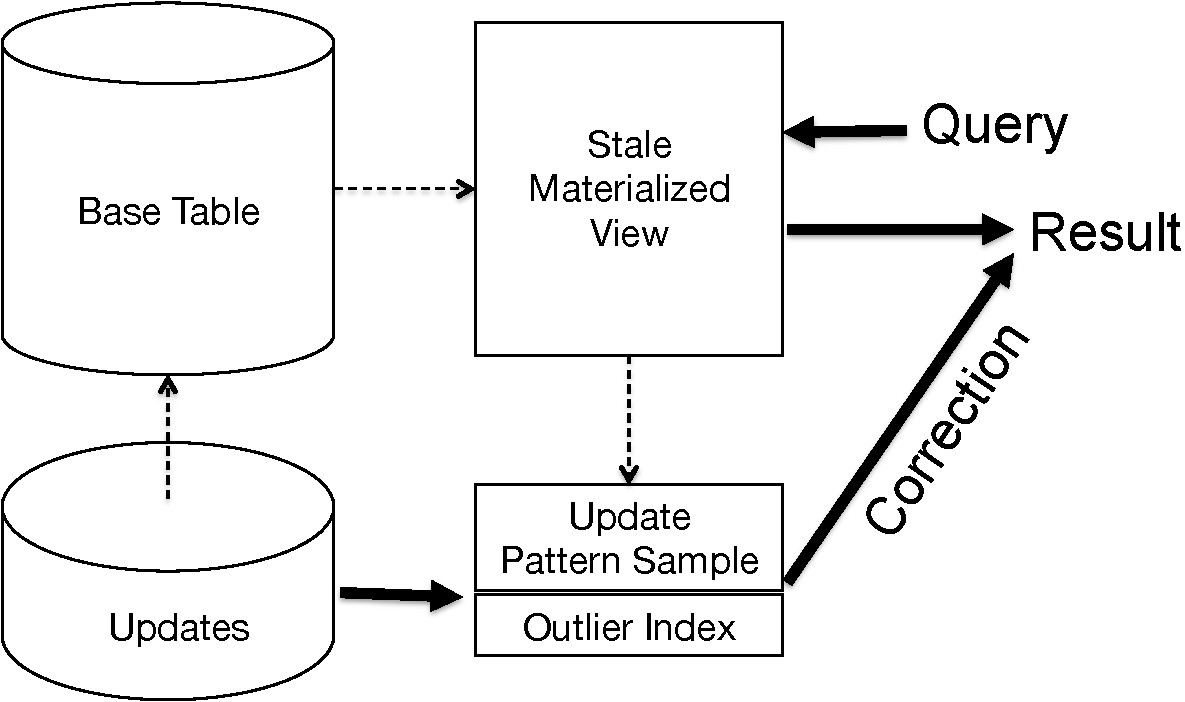
\includegraphics[scale=0.30]{figs/sys-arch.pdf}
 \caption{SVC has three main components: (1) sampling, (2) correction, and (3) outlier indexing. From a sample of up-to-date data, we estimate
 a correction for queries on stale MVs. To make this process robust to outliers, we apply a technique called outlier indexing. \label{sys-arch}}\vspace{-1.5em}
\end{figure}

Data cleaning has been studied extensively in the literature (e.g., see Rahm and Do for a survey\cite{rahm2000data}) but increasing data volumes and arrival rates have lead to development of new, efficient sampling-based approaches coping with dirty data.   In particular, the SampleClean framework has been shown to greatly improve query accuracy while cleaning a small sample of dirty records rather than an entire dirty data set \cite{wang1999sample}.  This data-cleaning perspective raises a new possibility for MVs, namely, that we can return more accurate results without incurring the cost of full view maintenance.   Of course, the metaphor of stale MVs as dirty data only goes so far. Staleness is different sort of data error that raises interesting new challenges in sampling, cleaning, and efficient query processing.

To address these challenges, we propose Sample-View-Clean (SVC), a framework that uses a \emph{sample} of up-to-date data to \emph{correct} stale query results.  While approximate, the corrected query result can be bounded within confidence intervals.
SVC is complementary to existing deferred maintenance approaches; when the MVs are stale between maintenance cycles, we can apply SVC for approximate results for a far smaller cost than having to maintain the entire view.
SVC gives results that are fresh, with a bounded approximation error that can be controlled by adjusting sampling ratio.


In Figure \ref{sys-arch}, we highlight the three main components of SVC: (1) sampling, (2) correction, and (3) outlier indexing. For (1), we define the notion of an ``update pattern", which represents how an update affects the view and we sample based on these patterns. For (2) we use the sample to estimate impact of the updates on the query result and we use this estimate to correct the stale query result.
Finally, in (3), since sampling is known to be sensitive to outliers (i.e., rows that have abnormal attribute values) \cite{chaudhuri2001overcoming}, we
utilize a technique called outlier indexing \cite{chaudhuri2001overcoming} to ensure that MV rows that are derived from an ``outlier" records are contained in the sample.  This technique further increases correction accuracy.

To summarize, our contributions are as follows:
\begin{itemize}\vspace{-.45em}
\item We model the incremental maintenance problem as a data cleaning problem and staleness as a type of data error.\vspace{-.45em}
\item We define the concept of ``update patterns", a logical unit that represents how an update affects a MV, and show how to sample the update patterns. \vspace{-.45em}
\item Using a sample of update patterns, we can correct stale aggregation queries on MVs with bounded accuracy.\vspace{-.45em}
\item We use an outlier index to increase the accuracy of the approach for power-law, long-tailed, and skewed distributions.\vspace{-.45em}
\item We evaluate our approach on a single node MySQL database with a 10GB skewed TPCD benchmark dataset and in a 20-node Apache Spark cluster with a 1TB log dataset from a video streaming company, Conviva. Our results suggest that sampling is significantly faster than full view maintenance, and also can give highly accurate results for a variety of queries and views.\vspace{-.45em}
\end{itemize}

The paper is organized as follows: 
In Section~\ref{sec-background}, we introduce MVs and discuss the current maintenance challenges.
Next, in Section~\ref{sec-arch}, we give a brief overview of our overall system architecture.
In Section~\ref{sampling} and~\ref{correction}, we describe the sampling and query processing of our technique.
In Section~\ref{outlier}, we describe the outlier indexing framework.
In Section~\ref{sec:ext}, we discuss how SVC extends to Select queries and deletions.
Then, in Section~\ref{exp}, we evaluate our approach.
Finally, we discuss Related Work in Section~\ref{related} and present our Conclusions and Future Work in Section~\ref{conclusion}.
